\documentclass{article}
\usepackage{float}
\usepackage{amsmath,amssymb,amsthm,graphicx}
\usepackage{subcaption}
\usepackage{mleftright}


\setlength{\oddsidemargin}{0.25 in}
\setlength{\evensidemargin}{-0.25 in}
\setlength{\topmargin}{-0.6 in}
\setlength{\textwidth}{6.5 in}
\setlength{\textheight}{8.5 in}
\setlength{\headsep}{0.75 in}
\setlength{\parindent}{0 in}
\setlength{\parskip}{0.1 in}

\newtheorem{theorem}{Theorem}
\newtheorem{corollary}{Corollary}
\newtheorem{proposition}{Proposition}
\newtheorem*{remark}{Remark}
\theoremstyle{definition}
\newtheorem{example}{Example}
\newtheorem{definition}{Definition}

\newcommand{\lecture}[4]{
   \pagestyle{myheadings}
   \thispagestyle{plain}
   \newpage
%   \setcounter{lecnum}{#1}
   \setcounter{page}{1}
   \noindent
   \begin{center}
   \framebox{
      \vbox{\vspace{2mm}
    \hbox to 6.58in { {\bf CSC~565: Graph Theory
                        \hfill North Carolina State University} }
    \hbox to 6.58in { {\bf Fall 2019
                        \hfill Computer Science} }
       \vspace{4mm}
       \hbox to 6.28in { {\Large \hfill Lecture #1: #2  \hfill} }
       \vspace{2mm}
       \hbox to 6.28in { {\it Lecturer: {\it Don Sheehy {\tt <drsheehy@ncsu.edu>}} \hfill Scribe: #4} }
      \vspace{2mm}}
   }
   \end{center}
   \markboth{Lecture #1: #2}{Lecture #1: #2}
   \vspace*{4mm}
}


\begin{document}
    \lecture{23}{Nov 11, 2019}{}{K. Alvarez, G. Hauser, C. Nelson, M. Riahi}

    \section{Overview}
    Consider the idea of surrealism, a literary and art movement in the early 20th century. In André Breton's Surrealist Manifestos, one of the starting points of surrealism was to do such things as interpret dreams and practice automatic writing to tap into the subconscious for flashes of insight. For instance, Salvador Dalí's art used a method called the Critical Paranoiac Method where he would catch himself in the first phase of hallucinatory sleep to gather images and ideas. These may include ideas where a figure is inside or outside another figure or a figure is comprised of other figures. Dalí would simply perfect it in his art to make it reality.
    \newline
    \newline
    In terms of algebraic graph theory, we can loosely use the idea of surrealism to ask ourselves: "How can I transform my matrix in a way that I can say something about it in a different form (i.e. applying computations on it)?" Since linear algebra is the study of vector spaces and linear transformations, we can view a matrix generated from a graph as a linear transformation and say something about it without thinking of the matrix as just a bunch of numbers.
    \newline
    \newline
    In this lecture, we continue from last lecture on algebraic graph theory and explore matrices as linear transformations and what we can do with these transformations.
    
    \section{Matrices as Linear Transformations}
    Let's think of matrices as transformations and not as numbers, rows, and columns. For example, to map the n-dimensional geometric realization of graph G into the plane (2D), we can write this as an $R^{n\times2}$ matrix $S$ where

    $$S =
        \left[ {\begin{array}{cccccccc}
            X_{1} & Y_{1} \\
            . & . \\
            . & . \\
            X_{n} & Y_{n} \\
        \end{array} } \right]
    \in R^{n\times2}$$

    and $S^T: R^n \rightarrow R^2$. Here, this gives us a linear transformation that preserves the fact that the edges are straight. We know this through geometric realization that if you take two vertices and the line segment between them, when you map them, any point on the line segment from $R^n \rightarrow R^2$ maps to another line segment.

    \subsection{Is it meaningful to treat adjacency matrices as a linear transformation? What is it doing? What can it transform into?}
    
    Recall that $A$ is the adjacency matrix of graph $G$ where
    
    $$A_{i,j} = [A]_{i,j} =
        \left\{
            \begin{array}{ll}
                1\hspace{1cm} if(i,j) \in E_G\\
                0\hspace{1cm} o/w\\
            \end{array}
        \right.$$

The mapping of $G\longmapsto A$ can be thought of as a graph invariant as long as there are equivalences in the space of matrices ``up to matrix similarity.''

Let's assume more transformations of matrices, where $A$ is a linear mapping between vector space $u$ and $M$ and $M^{-1}$ are linear mappings from $v$ to $u$ and $u$ to $v$ respectively. Then the composition of linear transformations gives us another linear transformation $M^{-1}AM$ between vector space $v$.  

\begin{figure}[H]
\centering
  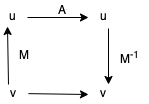
\includegraphics[width=0.2\columnwidth]{Images/p1.png}
  \caption{$A$ is acting on some vector. In $M^{-1}AM$, M transforms vector $v$ into another space $u$, applies A to $u$, and transforms it back to $v$.   }~\label{fig:figure1}
\end{figure}

\subsection{What can we do with the adjacency matrix as a linear transformation?}

\textbf{Lemma:} Assume $A$ is the adjacency matrix of the graph $G$, then we have $[A^k]_{i,j}=$ number of walks if length k from i to j. 

\textbf{Proof:} Induction on k
\\ Base: $A^0=I$ \checkmark $A^1$ \checkmark
\\ Hypothesis: $A^k= A^{k-1}\times A$
\\ \\ If we learn the way $A^k$ is made from $A^{k-1}$, and how A transforms $A^{k-1}$, we can prove the lemma for $A^{k+1}$ where the number of k-walks from i to j = $$\sum_{v \backsim i}^{} [A^{k-1}]_{v_j} = \sum_{v=1}^{n} A_{iv} \times [A^{k-1}]_{v_j}= [A A^{k-1}]_{i,j} = [A^K]_{i,j}$$
 
We can also prove it the same way for k+1-walks from i to j as well.

\textbf{Definition:} trace($M$) = $\sum_{i=1}^{n} M_{i,i} $   
\\ \textbf{Note:} The trace of a matrix is a graph invariant. Permuting rows and columns does not change the trace.

\textbf{Example}: 
\\ Assume $A$ is a matrix. Then the number of all walks of length 2 from a vertex to itself is
$$trace(A^2) = \sum_{i=1}^{n} A^2_{i,i} = \sum_{i=1}^{n} deg(i) = 2|E|$$ 

Similarly, we can define trace($A^3$) as the number of all walks of length 3 from a vertex to itself.

If $t$ = number of triangles ($K_3$ subgraphs) in a graph, for each vertex in a triangle there are 2 different walks of length 3 within the triangle. Since there are 3 vertices in each triangle, the total number of walks of the length 3 from a vertex to itself is equal to 6 times the number of triangles. Therefore,
$$trace(A^3) = 6\times t$$

where t = number of triangles ($K_3$ subgraphs) $\rightarrow$ \textit{graph invariant}

\section{Reminder: Eigenvalue and Eigen Vector}
A more interesting invariant can be found by learning eigenvalue and eigenvector of matrices.

\textbf{Definition:} ($\lambda$, v) is an eigenvalue, eigenvector pair of $M \in R^{n x n}$ if $Mv = \lambda v$.  

Suppose $A$ and $B$ are two similar matrices, and $M$ is the similarity transformation matrix $A = M^{-1}BM$. If $\lambda$ is an eigenvalue of $B$, then $\lambda$ is also an eigenvalue of $A$.
    
    \textbf{Proof:} 
    \\ Assume $Bv = \lambda v$ and $x = M^{-1}v$. Then $$Ax = M^{-1}BMM^{-1}v = M^{-1}Bv = \lambda M^{-1}v = \lambda x$$.
    
\textbf{Definition:} A sorted list of eigenvalues is called the \textbf{spectrum}.    

\subsection{How to we find an eigenvalue and eigenvector pair in a matrix?}

 Assume $Mv = \lambda v$. Then $$Mv - \lambda v = 0 \implies (M - \lambda I)v = 0$$. \\ Based on what was derived, it looks like that we have a linear system; however, $\lambda$ and $v$ are unknown and we need to know what they are. To solve this, we can take the determinant of the left hand side to determine if there is a nontrivial solution to this equation when 0 is on the right hand side.
 $$det(M - \lambda I) \leftarrow \text{char. polynomial roots are eigenvalues} \doteq 0.$$
 
\textbf{Small Example}  

 \[
   F=
  \left[ {\begin{array}{cccc}
   0 & 1 \\
   1 & 1 \\

  \end{array} } \right]
\]

Now we want to compute the $det(F - \lambda I)$, where $\lambda$s represent eigenvalues =  \[
  \left[ {\begin{array}{cccc}
   0-\lambda & 1 \\
   1 & 1-\lambda \\

  \end{array} } \right]
  = - \lambda (1-\lambda) -1 = \lambda^2 - \lambda -1 = 0
\]

Using the quadratic formula, $\lambda = \frac{1 \pm \sqrt{5}}{2}$

\textbf{Note:} $F$ has a special characteristic that multiplying it by
    $F \times \left[ \begin{array}{cc}
        0 \\
        1
    \end{array} \right]$,
generates Fibonacci numbers: \\
\[ F \times  \left[ \begin{array}{cc}
0 \\
1
\end{array} \right]
%
= 
\left[ \begin{array}{cc}
1 \\
1
\end{array} \right]
\hspace{0.5 cm}
%
F \times \left[ \begin{array}{cc}
1 \\
1
\end{array} \right]
%
= \left[ \begin{array}{cc}
1 \\
2
\end{array} \right] \hspace{0.5 cm}
%
F \times \left[ \begin{array}{cc}
1 \\
2
\end{array} \right]
%
= \left[ \begin{array}{cc}
2 \\
3 
\end{array} \right] \hspace{0.5 cm}
%
F \times \left[ \begin{array}{cc}
2 \\
3
\end{array} \right]
%
= \left[ \begin{array}{cc}
3 \\
5 
\end{array} \right]\]

%
In general: \[F^k \times \left[ \begin{array}{cc}
0 \\
1
\end{array} \right]
%
= \left[ \begin{array}{cc}
f_k \\
f_{k+1} 
\end{array} \right]
\]

\section{Matrices as functions}
Assume $M \in R^{n\times n}$ is a matrix. $u$ and $v$ are a pair of vectors that we want to map to matrix $M$.

Suppose $(u,v) \mapsto u^T M v$. Then $$(u,v) \mapsto u^T M v = \sum_{i=1}^{n} \sum_{j=1}^{n} M_{i,j} u_i v_j$$


$$ \left[ \begin{array}{ccccc}
u_1 \\
u_2 \\
. \\
.\\
u_n
\end{array} \right] ^T
\times  \left[ \begin{array}{ccccc}
 & & & & \\
 & & & & \\
  & & M& & \\
   & & & & \\
    & & & &
\end{array} \right]
%
\times
\left[ \begin{array}{ccccc}
v_1 \\
v_2\\ 
. \\
. \\
v_n
\end{array} \right]
$$

We can check that if $M = I$, then we have $u^T M v = u^T  v =  \sum_{i=1}^{n} u_i v_i$

\textbf{Note:} Bi-linearity is a nice property of this kind of mapping that uses the fact that matrices, as linear transformation, distribute over addition: 

$$<X,Y+Z>_M \rightarrow X^TM(Y+Z) \rightarrow X^T(MY+MZ) = X^TMY + X^TMZ = <X,Y>_M + <X,Z>_M$$

\section{Conclusion}
Assuming $G$ is a graph, we learned that a matrix $M$ can represent a linear transformations of $G$. Using $M$, we learned that we can extract information about $G$, like taking the power of the adjacency matrix gives information about the number of walks between certain vertices in a graph. We also discussed that in each linear transformation, there exists eigenvalue and eigenvector pairs that we can extract to obtain the spectral invariant of graphs. Finally, we discussed the idea that matrices can be treated as functions.

\end{document}